\documentclass[a4paper,12pt]{article} % добавить leqno в [] для нумерации слева
\usepackage[a4paper,top=1.3cm,bottom=2cm,left=1.5cm,right=1.5cm,marginparwidth=0.75cm]{geometry}
%%% Работа с русским языком
\usepackage{cmap}					% поиск в PDF
\usepackage[warn]{mathtext} 		% русские буквы в фомулах
\usepackage[T2A]{fontenc}			% кодировка
\usepackage[utf8]{inputenc}			% кодировка исходного текста
\usepackage[english,russian]{babel}	% локализация и переносы
\usepackage{physics}
\usepackage{multirow}
\usepackage{longtable}

%%% Нормальное размещение таблиц (писать [H] в окружении таблицы)
\usepackage{float}
\restylefloat{table}



\usepackage{graphicx}

\usepackage{wrapfig}
\usepackage{tabularx}

\usepackage{hyperref}
\usepackage[rgb]{xcolor}
\hypersetup{
	colorlinks=true,urlcolor=blue
}

\usepackage{pgfplots}
\pgfplotsset{compat=1.9}

%%% Дополнительная работа с математикой
\usepackage{amsmath,amsfonts,amssymb,amsthm,mathtools} % AMS
\usepackage{icomma} % "Умная" запятая: $0,2$ --- число, $0, 2$ --- перечисление

%% Номера формул
\mathtoolsset{showonlyrefs=true} % Показывать номера только у тех формул, на которые есть \eqref{} в тексте.

%% Шрифты
\usepackage{euscript}	 % Шрифт Евклид
\usepackage{mathrsfs} % Красивый матшрифт

%% Свои команды
\DeclareMathOperator{\sgn}{\mathop{sgn}}

%% Перенос знаков в формулах (по Львовскому)
\newcommand*{\hm}[1]{#1\nobreak\discretionary{}
	{\hbox{$\mathsurround=0pt #1$}}{}}

\date{\today}

\usepackage{gensymb}

\begin{document}

\begin{titlepage}
	\begin{center}
		{\large МОСКОВСКИЙ ФИЗИКО-ТЕХНИЧЕСКИЙ ИНСТИТУТ (НАЦИОНАЛЬНЫЙ ИССЛЕДОВАТЕЛЬСКИЙ УНИВЕРСИТЕТ)}
	\end{center}
	\begin{center}
		{\large Физтех-школа физики и исследований им. Ландау}
	\end{center}
	
	
	\vspace{4.5cm}
	{\huge
		\begin{center}
			{\bf Отчёт о выполнении лабораторной работы 2.4.1}\\
			Определение теплоты испарения жидкости
		\end{center}
	}
	\vspace{2cm}
	\begin{flushright}
		{\LARGE Автор:\\ Сенокосов Арсений Олегович \\
			\vspace{0.2cm}
			Б02-012}
	\end{flushright}
	\vspace{8cm}
	\begin{center}
		Долгопрудный\\
		\today
	\end{center}
\end{titlepage}


\section{Введение}
\textbf{Цель работы:}  \begin{enumerate}
	\item измерение давления насыщенного пара жидкости при разной температуре;
	\item вычисление по полученным данным теплоты испарения с помощью уравнения Клапейрона–Клаузиуса.
\end{enumerate}

\textbf{В работе используются:} термостат; герметический сосуд, заполненный исследуемой жидкостью; отсчетный микроскоп.

\section{Теоретические сведения}

Испарением называется переход вещества из жидкого в газообразное состояние. Оно происходит на свободной поверхности жидкости. При испарении с поверхности вылетают молекулы, образуя над ней пар. Для выхода из жидкости молекулы должны преодолеть силы молекулярного сцепления. Кроме того, при испарении совершается работа против внешнего давления $ P $, поскольку объем жидкости меньше объема пара. Не все молекулы жидкости способны совершить эту работу, а только те из них, которые обладают достаточной кинетической энергией. Поэтому переход части молекул в пар приводит к обеднению жидкости быстрыми молекулами, т.е. к ее охлаждению. Чтобы испарение проходило без изменения температуры, к жидкости нужно подводить тепло. Количество теплоты, необходимое для изотермического испарения одного моля жидкости при внешнем давлении, равном упругости ее насыщенных паров, называется молярной теплотой испарения (парообразования).

Теплоту парообразования жидкостей можно измерить непосредственно при помощи калориметра. Такой метод, однако, не позволяет получить точных результатов из-за неконтролируемых потерь тепла, которые трудно сделать малыми. В настоящей работе для определения теплоты испарения применен косвенный метод, основанный на формуле Клапейрона–Клаузиуса:

\begin{equation}\label{Kl-Kl}
\frac{dP}{dT}=\frac{L}{T\left(V_2-V_1\right)}.
\end{equation}

Здесь $ P $ -- давление насыщенного пара жидкости при температуре $ T $, $ T $ -- абсолютная температура жидкости и пара, $ L $ -- теплота испарения жидкости, $ V_2 $ -- объем пара, $ V_1 $ -- объем жидкости. Найдя из опыта $ dP/dT $, $ T $, $ V_2 $ и $ V_1 $, можно определить $ L $ путем расчета. Величины $ L $, $ V_2 $ и $ V_1 $ в формуле \eqref{Kl-Kl} должны относиться к одному и тому же количеству вещества; мы будем относить их к одному молю.

В нашем приборе измерения производятся при давлениях ниже атмосферного. В этом случае задача существенно упрощается.

При нашей точности опытов величиной $ V_1 $ в \eqref{Kl-Kl} можно пренебречь.

Обратимся теперь к $ V_2 $, которое в дальнейшем будем обозначать просто $ V $. Объем $ V $ связан с давлением и температурой уравнением Ван-дер-Ваальса:

\begin{equation}\label{VDV}
\left(P+\frac{a}{V^2}\right)\left(V-b\right)=RT.
\end{equation}

Из табличных данных следует, что $ b $ одного порядка с $ V_1 $. В уравнении Ван-дер-Ваальса величиной $ b $ следует пренебречь. Пренебрежение членом $ a/V^2 $ по сравнению с $ P $ вносит ошибку менее 3\%. При давлении ниже атмосферного ошибки становятся еще меньше. Таким образом, при давлениях ниже атмосферного уравнение Ван-дер-Ваальса для насыщенного пара мало отличается от уравнения Клапейрона. Положим поэтому

\begin{equation}\label{Volume}
V=\frac{RT}{P}.
\end{equation}

Подставляя \eqref{Volume} в \eqref{Kl-Kl}, пренебрегая $ V_1 $ и разрешая уравнение относительно $ L $, найдем

\begin{equation}\label{final}
L=\frac{RT^2}{P}\frac{dP}{dT}=-R\frac{d(\ln P)}{d(1/T)}.
\end{equation}

В нашем опыте температура жидкости измеряется термометром, давление пара определяется при помощи манометра, а производные $ dP/dT $ или $ d(\ln P)/d(1/T) $ находятся графически как угловой коэффициент касательной к кривой $ P(T) $ или соответственно к кривой, у которой по оси абсцисс отложено $ 1/T $, а по оси ординат $ \ln P $.

\section{Экспериментальная установка}

\begin{wrapfigure}{r}{6.5cm}
	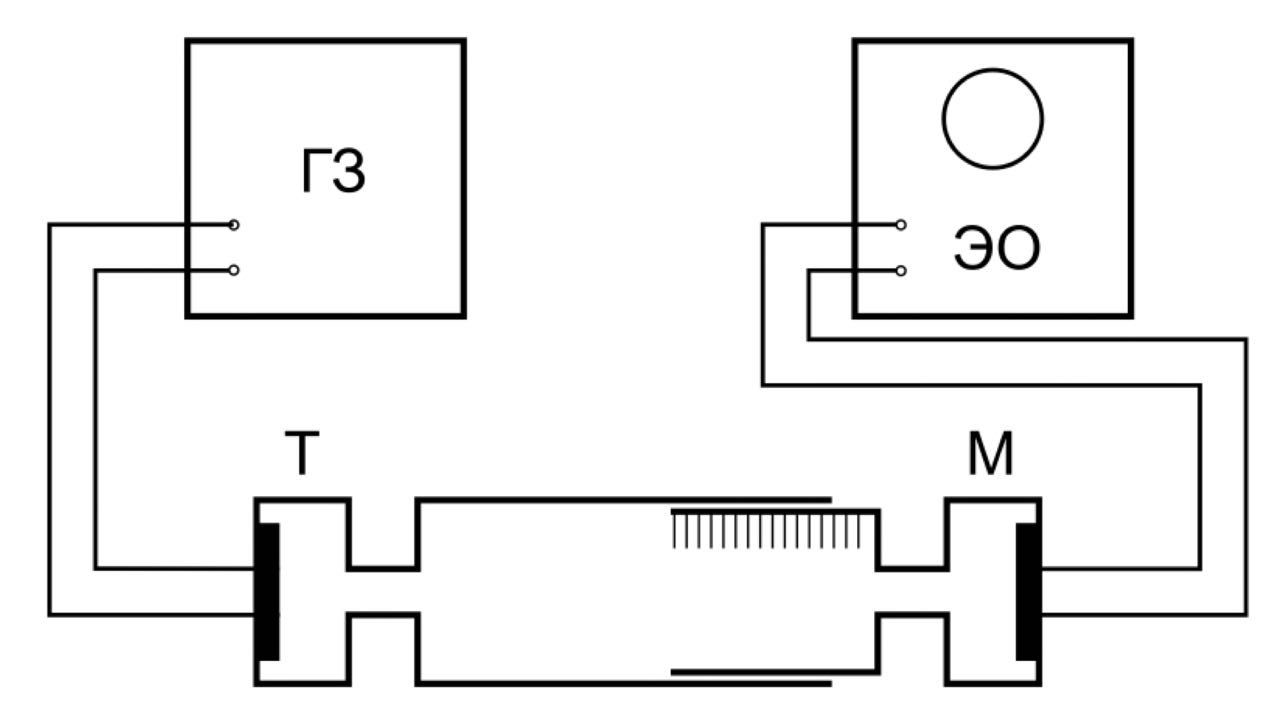
\includegraphics[width=6.5cm]{ust1.jpg}
	\caption{\textit{Схема первой установки}}
	\label{img1}
\end{wrapfigure}

Схема установки изображена на рисунке \ref{img1}. Наполненный водой резервуар 1 играет роль термостата. Нагревание термостата производится спиралью 2, подогреваемой электрическим током. Для охлаждения воды в термостате через змеевик 3 пропускается водопроводная вода. Вода в термостате перемешивается воздухом, поступающим через трубку 4. Температура воды измеряется термометром 5. В термостат погружен запаянный прибор 6 с исследуемой жидкостью. Над ней находится насыщенный пар (перед заполнением прибора воздух из него был откачан). Давление насыщенного пара определяется по ртутному манометру, соединенному с исследуемым объемом. Отсчет показаний манометра производится при помощи микроскопа.

На рисунке \ref{img2} приведена более полная схема такой же установки, но с использованием современного термостата. Установка включает термостат A, экспериментальный прибор B и отсчетный микроскоп C.

Экспериментальный прибор B представляет собой емкость 12, заполненную водой. В нее погружен запаянный прибор 13 с исследуемой жидкостью 14. Перед заполнением исследуемой жидкости воздух из запаянного прибора был удален, так что над жидкостью находится только её насыщенный пар. Давление пара определяется по ртутному манометру 15, соединенному с емкостью 13. Численная величина давления измеряется по разности показаний отсчетного микроскопа 16, настраиваемого последовательно на нижний и верхний уровни столбика ртути манометра. Показания микроскопа снимаются по шкале 17.

Описание прибора указывает на второе важное преимущество предложенного косвенного метода измерения $ L $ перед прямым. При непосредственном измерении теплоты испарения опыты нужно производить при неизменном давлении, и прибор не может быть запаян. При этом невозможно обеспечить такую чистоту и неизменность экспериментальных условий, как при нашей постановке опыта.

Описываемый прибор обладает важным недостатком: термометр определяет температуру термостата, а не исследуемой жидкости (или ее пара). Эти температуры близки друг к другу лишь в том случае, если нагревание происходит достаточно медленно. Убедиться в том, что темп нагревания не является слишком быстрым, можно, сравнивая результаты, полученные при нагревании и при остывании прибора. Такое сравнение необходимо сделать. Для ориентировки укажем, что температуру воды в калориметре следует менять не быстрее, чем на 1 $ ^\circ C $ в течение 1–3 минут.

\begin{figure}[H]
\begin{center}
		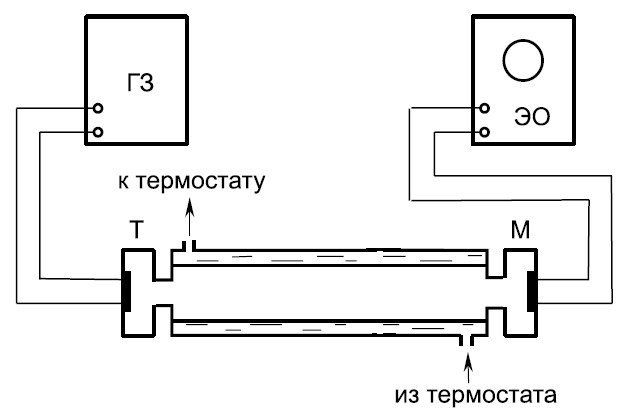
\includegraphics[width=15cm]{ust2.jpg}
\end{center}
	\caption{\textit{Схема второй установки}}
	\label{img2}
\end{figure}

\section{Ход работы}

\subsection{Проведение измерений}

Для определения теплоты парообразования воды измерим давление насыщенного пара при различных значениях температуры. Давление определяем при помощи ртутного манометра. При помощи штангенциркуля находим высоты $ h_1 $ и $ h_2 $ ртутных столбиков и по формуле  \begin{equation}\label{P}
\Delta P = \rho g (h_1 - h_2)
\end{equation}  находим давление насыщенного пара при определённой температуре. Результаты измерений заносим в таблицу \ref{tab:measures}.

При оценки погрешности измерения давления по формуле \eqref{P} следует использовать следующие соотношения:
\[ \sigma^2_{A\pm B} = \sigma^2_A+\sigma^2_B, \]
\[ \varepsilon^2_{A\cdot B} = \varepsilon^2_A+\varepsilon^2_B. \]

Также на моей установке поверх столбика ртути был столб воды высотой $ h' \approx 53,4 $ мм. Ввиду значительной высоты столба жидкости следует сделать поправку на это добавочное давление. Занесём в таблицу \ref{tab:measures} скорректированное значение давления насыщенного пара, вычисленное по формуле \[ \Delta P' = \Delta P + \rho_\text{в}gh', \] где $ h' $ -- высота столбика воды.

Используя перечисленные выше формулы, получаем, что погрешность измерения давления для каждого измерения составляет $ \sigma \approx 9,4 $ Па. ($ \varepsilon \approx 0,2 \% $). Таким образом, для определения теплоты парообразования будем использовать значения давления насыщенного пара, вместе с поправкой, описанной выше. (т.е. из столбца $ \Delta P' $)

\begin{table}[H]
	\centering
	\begin{tabular}{|c|c|c|c|c|c|c|c|c|c|c|}
		\cline{1-5} \cline{7-11}
		\multicolumn{5}{|c|}{Нагрев} &  & \multicolumn{5}{c|}{Охлаждение} \\ \cline{1-5} \cline{7-11} 
		$ T $, К & $ h_1 $, мм & $ h_2 $, мм & $ \Delta P $, Па & $ \Delta P' $, Па &  & $ T $, К & $ h_1 $, мм & $ h_2 $, мм & $ \Delta P $, Па & $ \Delta P' $, Па \\ \cline{1-5} \cline{7-11} 
		293,2 & 99,00 & 80,30 & 2485,0 & 3007,8 &  & 293,2 & 99,30 & 80,00 & 2564,7 & 3087,5 \\ \cline{1-5} \cline{7-11} 
		294,0 & 99,10 & 80,20 & 2511,6 & 3034,4 &  & 294,0 & 99,60 & 79,70 & 2644,4 & 3167,2 \\ \cline{1-5} \cline{7-11} 
		295,0 & 99,25 & 80,05 & 2551,4 & 3074,2 &  & 295,0 & 100,20 & 79,10 & 2803,9 & 3326,7 \\ \cline{1-5} \cline{7-11} 
		296,0 & 99,95 & 79,35 & 2737,5 & 3260,3 &  & 296,0 & 100,70 & 78,60 & 2936,8 & 3459,6 \\ \cline{1-5} \cline{7-11} 
		297,0 & 100,75 & 78,55 & 2950,1 & 3472,9 &  & 297,0 & 101,40 & 77,90 & 3122,8 & 3645,6 \\ \cline{1-5} \cline{7-11} 
		298,0 & 101,40 & 77,90 & 3122,8 & 3645,6 &  & 298,0 & 102,10 & 77,20 & 3308,9 & 3831,7 \\ \cline{1-5} \cline{7-11} 
		299,0 & 102,15 & 77,15 & 3322,2 & 3845,0 &  & 299,0 & 102,80 & 76,50 & 3494,9 & 4017,7 \\ \cline{1-5} \cline{7-11} 
		300,0 & 102,95 & 76,35 & 3534,8 & 4057,6 &  & 300,0 & 103,60 & 75,70 & 3707,5 & 4230,3 \\ \cline{1-5} \cline{7-11} 
		301,0 & 103,80 & 75,50 & 3760,7 & 4283,5 &  & 301,0 & 104,50 & 74,80 & 3946,7 & 4469,5 \\ \cline{1-5} \cline{7-11} 
		302,0 & 104,60 & 74,70 & 3973,3 & 4496,1 &  & 302,0 & 105,30 & 74,00 & 4159,3 & 4682,1 \\ \cline{1-5} \cline{7-11} 
		303,0 & 105,35 & 73,95 & 4172,6 & 4695,4 &  & 303,0 & 106,10 & 73,20 & 4372,0 & 4894,8 \\ \cline{1-5} \cline{7-11} 
		304,0 & 106,40 & 72,90 & 4451,7 & 4974,5 &  & 304,0 & 106,70 & 72,60 & 4531,4 & 5054,2 \\ \cline{1-5} \cline{7-11} 
		305,0 & 107,10 & 72,20 & 4637,7 & 5160,5 &  & 305,0 & 107,80 & 71,50 & 4823,8 & 5346,6 \\ \cline{1-5} \cline{7-11} 
		306,0 & 108,20 & 71,10 & 4930,1 & 5452,9 &  & 306,0 & 108,90 & 70,40 & 5116,1 & 5638,9 \\ \cline{1-5} \cline{7-11} 
		307,0 & 109,20 & 70,10 & 5195,9 & 5718,7 &  & 307,0 & 109,90 & 69,40 & 5381,9 & 5904,7 \\ \cline{1-5} \cline{7-11} 
		308,0 & 109,90 & 69,40 & 5381,9 & 5904,7 &  & 308,0 & 111,20 & 68,10 & 5727,4 & 6250,2 \\ \cline{1-5} \cline{7-11} 
		309,0 & 110,75 & 68,55 & 5607,8 & 6130,6 &  & 309,0 & 111,90 & 67,40 & 5913,4 & 6436,2 \\ \cline{1-5} \cline{7-11} 
		310,0 & 112,10 & 67,20 & 5966,6 & 6489,4 &  & 310,0 & 113,00 & 66,30 & 6205,8 & 6728,6 \\ \cline{1-5} \cline{7-11} 
		311,0 & 113,30 & 66,00 & 6285,5 & 6808,3 &  & 311,0 & 114,20 & 65,10 & 6524,7 & 7047,5 \\ \cline{1-5} \cline{7-11} 
		312,0 & 114,70 & 64,60 & 6657,6 & 7180,4 &  & 312,0 & 115,20 & 64,10 & 6790,5 & 7313,3 \\ \cline{1-5} \cline{7-11} 
		313,0 & 116,10 & 63,20 & 7029,7 & 7552,5 &  & 313,0 & 116,10 & 63,20 & 7029,7 & 7552,5 \\ \cline{1-5} \cline{7-11} 
	\end{tabular}
	\caption{Измерение зависимости давления насыщенного пара от температуры жидкости}
	\label{tab:measures}
\end{table}

\subsection{Определение теплоты парообразования по графику $ P(T) $}

По данным из таблицы \ref{tab:measures} построим график зависимости давления насыщенного пара от температуры.

\begin{figure}[H]
	
	\begin{center}
		\begin{tikzpicture}
		\begin{axis}[
		/pgf/number format/.cd, use comma, 1000 sep = {},
		title={График зависимости $ P \left( T \right) $.},
		xlabel={$ T $, \textdegree К},
		ylabel={$ P $, Па},
		legend pos=north west,
		xmajorgrids=true,
		ymajorgrids=true,
		grid style=dashed,
		width = 495,
		height = 280,
		%xmin = 300,
		%xmax = 335,
		%ymin =40,
		%ymax =135,
		]
		\legend{ 
			Нагрев,
			Охлаждение,
		};
		\addplot+ [color=black, only marks, mark size = 3pt, mark options = {
	fill = red,
	draw = black,	
	},
		error bars/.cd,
		x dir=both, x explicit,
		y dir=both, y explicit, 
		] table [x = T, y = P, x error = dT, y error = dP,] {
			T	dT	P	dP                  
			293.2	0.10	3007.779354	9.421945032
			294.0	0.10	3034.356606	9.421945032
			295.0	0.10	3074.222484	9.421945032
			296.0	0.10	3260.263248	9.421945032
			297.0	0.10	3472.881264	9.421945032
			298.0	0.10	3645.633402	9.421945032
			299.0	0.10	3844.962792	9.421945032
			300.0	0.10	4057.580808	9.421945032
			301.0	0.10	4283.48745	9.421945032
			302.0	0.10	4496.105466	9.421945032
			303.0	0.10	4695.434856	9.421945032
			304.0	0.10	4974.496002	9.421945032
			305.0	0.10	5160.536766	9.421945032
			306.0	0.10	5452.886538	9.421945032
			307.0	0.10	5718.659058	9.421945032
			308.0	0.10	5904.699822	9.421945032
			309.0	0.10	6130.606464	9.421945032
			310.0	0.10	6489.399366	9.421945032
			311.0	0.10	6808.32639	9.421945032
			312.0	0.10	7180.407918	9.421945032
			313.0	0.10	7552.489446	9.421945032	
		};
		\addplot+ [color=black, only marks, mark size = 3pt, mark options = {
			fill = blue,
			draw = black,}	,
		error bars/.cd,
		x dir=both, x explicit,
		y dir=both, y explicit, 
		] table [x = T, y = P, x error = dT, y error = dP,] {
			T	dT	P	dP                  
			293.2	0.10	3087.51111	9.421945032
			294	0.10	3167.242866	9.421945032
			295	0.10	3326.706378	9.421945032
			296	0.10	3459.592638	9.421945032
			297	0.10	3645.633402	9.421945032
			298	0.10	3831.674166	9.421945032
			299	0.10	4017.71493	9.421945032
			300	0.10	4230.332946	9.421945032
			301	0.10	4469.528214	9.421945032
			302	0.10	4682.14623	9.421945032
			303	0.10	4894.764246	9.421945032
			304	0.10	5054.227758	9.421945032
			305	0.10	5346.57753	9.421945032
			306	0.10	5638.927302	9.421945032
			307	0.10	5904.699822	9.421945032
			308	0.10	6250.204098	9.421945032
			309	0.10	6436.244862	9.421945032
			310	0.10	6728.594634	9.421945032
			311	0.10	7047.521658	9.421945032
			312	0.10	7313.294178	9.421945032
			313	0.10	7552.489446	9.421945032	
		};
	\addplot [red, domain=292.5:313.5, line width = 2.2pt] {0.002208895 * e^(0.048064765 * x)};
	\addplot [blue, domain=292.5:313.5, line width = 2.2pt] {0.003518237 * e^(0.046658639 * x)};
		\end{axis}
		\end{tikzpicture}
	\end{center}
	
\end{figure}

Аппроксимируем методом наименьших квадратов полученные на этом участке температур зависимости функциями вида \[ P=ae^{bT}, \] где $ a $ и $ b $ -- неизвестные параметры. Используем следующие формулы:

\[ b = \frac{\langle \ln P \cdot T \rangle - \langle T \rangle \langle \ln P \rangle}{\langle T^2 \rangle - \langle T \rangle ^2},\]
\[ \ln a = \langle \ln P \rangle - b\langle T \rangle. \]

Случайные погрешности вычисления этих величин находим по следующим формулам:

\[ \sigma^\text{случ}_b = \sqrt{\frac{1}{N-2} \left(\frac{\left\langle\left(\ln P - \langle \ln P\right\rangle\right)^2 \rangle}{\left\langle\left(T - \langle T\right\rangle\right)^2 \rangle}\right)-b^2},\]
\[ \sigma^\text{случ}_{\ln a}=\sigma^\text{случ}_b\sqrt{\left\langle T^2 \right\rangle}. \]

\label{mnk}

Вкладом систематической погрешности в общую можно пренебречь в виду её малости по сравнению со случайной погрешностью определения коэффициентов. Поэтому будем считать, что \[ \sigma_b \approx \sigma^\text{случ}_b, \] \[ \sigma_{\ln a} \approx \sigma^\text{случ}_{\ln a}. \]

Полученные результаты заносим в таблицу \ref{tab:ab} и наносим зависимости на график.

\begin{table}[H]
	\centering
	\begin{tabular}{|c|c|c|c|c|}
		\hline
		Опыт & $ a \cdot 10^{-3}$, Па & $ \sigma_a \cdot 10^{-3}$, Па & $ b \cdot 10^{-2} $, К$ ^{-1} $ & $ \sigma_b \cdot 10^{-2} $, К$ ^{-1} $ \\ \hline
		нагрев & 2,21 & 0,34 & 4,81 & 0,05 \\ \hline
		охлаждение & 3,52 & 0,38 & 4,67 & 0,04 \\ \hline
	\end{tabular}
	\caption{Определение коэффициентов зависимости}
	\label{tab:ab}
\end{table}

Используя полученные результаты, можно получить формулу для производной давления по температуру: 
\begin{equation}\label{dpdt}
\frac{dP}{dT} = abe^{bT}.
\end{equation}
Подставляя \eqref{dpdt} в \eqref{final}, получаем:
\begin{equation}\label{newFinal}
L=\frac{RT^2ab}{P}e^{bT}.
\end{equation}

По полученным выше формулам вычисляем теплоту парообразования воды. Погрешность вычисления этой величины можно оценить по следующим формулам:
\[ \sigma_L = L\varepsilon_{\frac{dP}{dT}}, \]
\[ \sigma_{\frac{dP}{dT}} = \sqrt{\left(\frac{\partial\frac{dP}{dT}}{\partial a}\sigma_a\right)^2+\left(\frac{\partial\frac{dP}{dT}}{\partial b}\sigma_b\right)^2} \]

Полученные результаты заносим в таблицу \ref{tab:par}.

Полученные в этой части работы значения затем сравним со значениями, которые будут получены другим методом в следующей части.

\begin{table}[H]
	\centering
	\begin{tabular}{|c|c|c|c|c|c|c|c|c|}
		\cline{1-4} \cline{6-9}
		\multicolumn{4}{|c|}{Нагрев} &  & \multicolumn{4}{c|}{Охлаждение} \\ \cline{1-4} \cline{6-9} 
		$ T $, К & $ P $, Па & $ L $, $ \frac{\text{кДж}}{\text{моль}} $ & $ \sigma_L $, $ \frac{\text{кДж}}{\text{моль}} $ &  & $ T $, К & $ P $, Па & $ L $, $ \frac{\text{кДж}}{\text{моль}} $ & $ \sigma_L $, $ \frac{\text{кДж}}{\text{моль}} $ \\ \cline{1-4} \cline{6-9} 
		293,2 & 3007,8 & 33,3 & 5,2 &  & 293,2 & 3087,5 & 33,2 & 3,7 \\ \cline{1-4} \cline{6-9} 
		294,0 & 3034,4 & 34,5 & 5,4 &  & 294,0 & 3167,2 & 33,8 & 3,7 \\ \cline{1-4} \cline{6-9} 
		295,0 & 3074,2 & 35,9 & 5,6 &  & 295,0 & 3326,7 & 33,9 & 3,8 \\ \cline{1-4} \cline{6-9} 
		296,0 & 3260,3 & 35,8 & 5,6 &  & 296,0 & 3459,6 & 34,4 & 3,8 \\ \cline{1-4} \cline{6-9} 
		297,0 & 3472,9 & 35,5 & 5,6 &  & 297,0 & 3645,6 & 34,4 & 3,8 \\ \cline{1-4} \cline{6-9} 
		298,0 & 3645,6 & 35,7 & 5,6 &  & 298,0 & 3831,7 & 34,6 & 3,8 \\ \cline{1-4} \cline{6-9} 
		299,0 & 3845,0 & 35,8 & 5,6 &  & 299,0 & 4017,7 & 34,8 & 3,9 \\ \cline{1-4} \cline{6-9} 
		300,0 & 4057,6 & 35,8 & 5,6 &  & 300,0 & 4230,3 & 34,8 & 3,9 \\ \cline{1-4} \cline{6-9} 
		301,0 & 4283,5 & 35,8 & 5,6 &  & 301,0 & 4469,5 & 34,8 & 3,9 \\ \cline{1-4} \cline{6-9} 
		302,0 & 4496,1 & 36,0 & 5,7 &  & 302,0 & 4682,1 & 35,0 & 3,9 \\ \cline{1-4} \cline{6-9} 
		303,0 & 4695,4 & 36,5 & 5,7 &  & 303,0 & 4894,8 & 35,3 & 3,9 \\ \cline{1-4} \cline{6-9} 
		304,0 & 4974,5 & 36,3 & 5,7 &  & 304,0 & 5054,2 & 36,1 & 4,0 \\ \cline{1-4} \cline{6-9} 
		305,0 & 5160,5 & 37,0 & 5,8 &  & 305,0 & 5346,6 & 36,0 & 4,0 \\ \cline{1-4} \cline{6-9} 
		306,0 & 5452,9 & 37,0 & 5,8 &  & 306,0 & 5638,9 & 36,0 & 4,0 \\ \cline{1-4} \cline{6-9} 
		307,0 & 5718,7 & 37,2 & 5,8 &  & 307,0 & 5904,7 & 36,2 & 4,0 \\ \cline{1-4} \cline{6-9} 
		308,0 & 5904,7 & 38,1 & 6,0 &  & 308,0 & 6250,2 & 36,1 & 4,0 \\ \cline{1-4} \cline{6-9} 
		309,0 & 6130,6 & 38,7 & 6,1 &  & 309,0 & 6436,2 & 36,9 & 4,1 \\ \cline{1-4} \cline{6-9} 
		310,0 & 6489,4 & 38,6 & 6,1 &  & 310,0 & 6728,6 & 37,3 & 4,1 \\ \cline{1-4} \cline{6-9} 
		311,0 & 6808,3 & 38,9 & 6,1 &  & 311,0 & 7047,5 & 37,5 & 4,2 \\ \cline{1-4} \cline{6-9} 
		312,0 & 7180,4 & 39,0 & 6,1 &  & 312,0 & 7313,3 & 38,1 & 4,2 \\ \cline{1-4} \cline{6-9} 
		313,0 & 7552,5 & 39,1 & 6,1 &  & 313,0 & 7552,5 & 38,9 & 4,3 \\ \cline{1-4} \cline{6-9} 
	\end{tabular}
	\caption{Результаты вычисления теплоты парообразования}
	\label{tab:par}
\end{table}

\subsection{Определение теплоты парообразования по графику $ \ln P $ от $ 1 / T $}

Для построения графика преобразуем данные из таблицы \ref{tab:measures}. Преобразованные результаты измерений занесём в таблицу \ref{tab:ln}. Полученные значения наносим на график.

\begin{figure}[H]
	
	\begin{center}
		\begin{tikzpicture}
		\begin{axis}[
		/pgf/number format/.cd, use comma, 1000 sep = {},
		title={График зависимости $ \ln P \left( 1/T \right) $.},
		xlabel={$ 1 / T \cdot 10^{-3} $, К$ ^{-1} $},
		ylabel={$ \ln P $},
		legend pos=north east,
		xmajorgrids=true,
		ymajorgrids=true,
		grid style=dashed,
		width = 495,
		height = 270,
		%xmin = 300,
		%xmax = 335,
		%ymin =40,
		%ymax =135,
		]
		\legend{ 
			Нагрев,
			Охлаждение,
		};
		\addplot+ [color=black, only marks, mark size = 3pt, mark options = {
			fill = red,
			draw = black,	
		}, 
		] table [x = T, y = P] {
			T	P                  
			3.410641201	8.008957329
			3.401360544	8.01775469
			3.389830508	8.030807298
			3.378378378	8.089563222
			3.367003367	8.152739864
			3.355704698	8.201285402
			3.344481605	8.254519205
			3.333333333	8.308342215
			3.322259136	8.362522782
			3.311258278	8.410966849
			3.300330033	8.454346008
			3.289473684	8.512079338
			3.278688525	8.548795877
			3.267973856	8.603900387
			3.25732899	8.651489626
			3.246753247	8.683503893
			3.236245955	8.721048958
			3.225806452	8.777925258
			3.215434084	8.825901611
			3.205128205	8.879111474
			3.194888179	8.929632516
				
		};
		\addplot+ [color=black, only marks, mark size = 3pt, mark options = {
			fill = blue,
			draw = black,}	,
		] table [x = T, y = P] {
			T	P               
			3.410641201	8.035120579
			3.401360544	8.06061673
			3.389830508	8.109738018
			3.378378378	8.148906126
			3.367003367	8.201285402
			3.355704698	8.251057106
			3.344481605	8.298468595
			3.333333333	8.35003598
			3.322259136	8.405038137
			3.311258278	8.45151188
			3.300330033	8.495921392
			3.289473684	8.527980352
			3.278688525	8.584211921
			3.267973856	8.637449132
			3.25732899	8.683503893
			3.246753247	8.740369398
			3.236245955	8.769700553
			3.225806452	8.81412158
			3.215434084	8.860431296
			3.205128205	8.897449091
			3.194888179	8.929632516
		};
	\addplot [red, domain=3.19:3.42, line width = 2.2pt] {23.0081996396733 -  4.40987806078315*x};
	\addplot [blue, domain=3.19:3.42, line width = 2.2pt] {22.6246675288121-4.28177716244523*x};
		\end{axis}
		\end{tikzpicture}
	\end{center}
	
\end{figure}

\begin{table}[H]
	\centering
	\begin{tabular}{|c|c|c|c|c|}
		\cline{1-2} \cline{4-5}
		\multicolumn{2}{|c|}{Нагрев} &  & \multicolumn{2}{c|}{Охлаждение} \\ \cline{1-2} \cline{4-5} 
		$ T \cdot 10^{-3} $, К$ ^{-1} $ & $ \ln P $ &  & $ T \cdot 10^{-3} $, К$ ^{-1} $ & $ \ln P $ \\ \cline{1-2} \cline{4-5} 
		3,411 & 8,009 &  & 3,411 & 8,035 \\ \cline{1-2} \cline{4-5} 
		3,401 & 8,018 &  & 3,401 & 8,061 \\ \cline{1-2} \cline{4-5} 
		3,390 & 8,031 &  & 3,390 & 8,110 \\ \cline{1-2} \cline{4-5} 
		3,378 & 8,090 &  & 3,378 & 8,149 \\ \cline{1-2} \cline{4-5} 
		3,367 & 8,153 &  & 3,367 & 8,201 \\ \cline{1-2} \cline{4-5} 
		3,356 & 8,201 &  & 3,356 & 8,251 \\ \cline{1-2} \cline{4-5} 
		3,344 & 8,255 &  & 3,344 & 8,298 \\ \cline{1-2} \cline{4-5} 
		3,333 & 8,308 &  & 3,333 & 8,350 \\ \cline{1-2} \cline{4-5} 
		3,322 & 8,363 &  & 3,322 & 8,405 \\ \cline{1-2} \cline{4-5} 
		3,311 & 8,411 &  & 3,311 & 8,452 \\ \cline{1-2} \cline{4-5} 
		3,300 & 8,454 &  & 3,300 & 8,496 \\ \cline{1-2} \cline{4-5} 
		3,289 & 8,512 &  & 3,289 & 8,528 \\ \cline{1-2} \cline{4-5} 
		3,279 & 8,549 &  & 3,279 & 8,584 \\ \cline{1-2} \cline{4-5} 
		3,268 & 8,604 &  & 3,268 & 8,637 \\ \cline{1-2} \cline{4-5} 
		3,257 & 8,651 &  & 3,257 & 8,684 \\ \cline{1-2} \cline{4-5} 
		3,247 & 8,684 &  & 3,247 & 8,740 \\ \cline{1-2} \cline{4-5} 
		3,236 & 8,721 &  & 3,236 & 8,770 \\ \cline{1-2} \cline{4-5} 
		3,226 & 8,778 &  & 3,226 & 8,814 \\ \cline{1-2} \cline{4-5} 
		3,215 & 8,826 &  & 3,215 & 8,860 \\ \cline{1-2} \cline{4-5} 
		3,205 & 8,879 &  & 3,205 & 8,897 \\ \cline{1-2} \cline{4-5} 
		3,195 & 8,930 &  & 3,195 & 8,930 \\ \cline{1-2} \cline{4-5} 
	\end{tabular}
	\caption{Зависимость $\ln P$ от $1/T$}
	\label{tab:ln}
\end{table}

С помощью формул, описанных в \ref{mnk}, вычислим значение и погрешность определения коэффициента $ \displaystyle \frac{d(\ln P)}{d(1/T)} $ с помощью метода наименьших квадратов. Таким образом, получаем

\[ \left(\frac{d(\ln P)}{d(1/T)}\right)_\text{нагр} = \left(-4410\pm48\right)\text{ К}, \]

\[ \left(\frac{d(\ln P)}{d(1/T)}\right)_\text{охл} = \left(-4282\pm27\right)\text{ К}. \]

По формуле \eqref{final} вычисляем теплоту парообразования. Получаем:

\[ L_\text{нагр} = \left(36,7 \pm 0,4\right) \text{ } \frac{\text{кДж}}{\text{моль}}, \]
\[ L_\text{охл} = \left(35,6 \pm 0,2\right) \text{ } \frac{\text{кДж}}{\text{моль}}. \]

Полученные значения будут сравнены с эталонными значениями и со значениями, полученными в предыдущей части работы, в п. \ref{res}.

\section{Обсуждение результатов и выводы}
\label{res}

В ходе выполнения работы:

\begin{itemize}
	\item была исследована зависимость давления насыщенных паров воды от давления жидкости;
	\item были вычислены теплоты парообразования воды для различных температур двумя разными способами.
\end{itemize}

Результаты по точечного вычисления теплоты парообразования по графику $ P(T) $ представлены в таблице \ref{tab:results}.

\begin{table}[H]
	\caption{Результаты измерений теплоты парообразования}
	\label{tab:results}
	\centering
	\begin{tabular}{|c|c|c|c|c|c|c|c|c|}
		\cline{1-4} \cline{6-9}
		\multicolumn{4}{|c|}{Нагрев} &  & \multicolumn{4}{c|}{Охлаждение} \\ \cline{1-4} \cline{6-9} 
		$ T $, К & $ L $, $ \displaystyle \frac{\text{МДж}}{\text{кг}} $ & $ \sigma_L $, $ \displaystyle\frac{\text{МДж}}{\text{кг}} $ & $ \varepsilon $, \% &  & $ T $, К & $ L $, $\displaystyle \frac{\text{МДж}}{\text{кг}} $ & $ \sigma_L $, $\displaystyle \frac{\text{МДж}}{\text{кг}} $ & $ \varepsilon $, \% \\ \cline{1-4} \cline{6-9} 
		293,2 & 1,85 & 0,29 & 15,7 &  & 293,2 & 1,84 & 0,20 & 11,1 \\ \cline{1-4} \cline{6-9} 
		294,0 & 1,91 & 0,30 & 15,7 &  & 294,0 & 1,88 & 0,21 & 11,1 \\ \cline{1-4} \cline{6-9} 
		295,0 & 2,00 & 0,31 & 15,7 &  & 295,0 & 1,88 & 0,21 & 11,1 \\ \cline{1-4} \cline{6-9} 
		296,0 & 1,99 & 0,31 & 15,7 &  & 296,0 & 1,91 & 0,21 & 11,1 \\ \cline{1-4} \cline{6-9} 
		297,0 & 1,97 & 0,31 & 15,7 &  & 297,0 & 1,91 & 0,21 & 11,1 \\ \cline{1-4} \cline{6-9} 
		298,0 & 1,98 & 0,31 & 15,7 &  & 298,0 & 1,92 & 0,21 & 11,1 \\ \cline{1-4} \cline{6-9} 
		299,0 & 1,99 & 0,31 & 15,7 &  & 299,0 & 1,93 & 0,21 & 11,1 \\ \cline{1-4} \cline{6-9} 
		300,0 & 1,99 & 0,31 & 15,7 &  & 300,0 & 1,93 & 0,21 & 11,1 \\ \cline{1-4} \cline{6-9} 
		301,0 & 1,99 & 0,31 & 15,7 &  & 301,0 & 1,93 & 0,21 & 11,1 \\ \cline{1-4} \cline{6-9} 
		302,0 & 2,00 & 0,31 & 15,7 &  & 302,0 & 1,94 & 0,22 & 11,1 \\ \cline{1-4} \cline{6-9} 
		303,0 & 2,03 & 0,32 & 15,7 &  & 303,0 & 1,96 & 0,22 & 11,1 \\ \cline{1-4} \cline{6-9} 
		304,0 & 2,02 & 0,32 & 15,7 &  & 304,0 & 2,00 & 0,22 & 11,1 \\ \cline{1-4} \cline{6-9} 
		305,0 & 2,06 & 0,32 & 15,7 &  & 305,0 & 2,00 & 0,22 & 11,1 \\ \cline{1-4} \cline{6-9} 
		306,0 & 2,05 & 0,32 & 15,7 &  & 306,0 & 2,00 & 0,22 & 11,1 \\ \cline{1-4} \cline{6-9} 
		307,0 & 2,07 & 0,32 & 15,7 &  & 307,0 & 2,01 & 0,22 & 11,1 \\ \cline{1-4} \cline{6-9} 
		308,0 & 2,12 & 0,33 & 15,7 &  & 308,0 & 2,00 & 0,22 & 11,1 \\ \cline{1-4} \cline{6-9} 
		309,0 & 2,15 & 0,34 & 15,7 &  & 309,0 & 2,05 & 0,23 & 11,1 \\ \cline{1-4} \cline{6-9} 
		310,0 & 2,15 & 0,34 & 15,7 &  & 310,0 & 2,07 & 0,23 & 11,1 \\ \cline{1-4} \cline{6-9} 
		311,0 & 2,16 & 0,34 & 15,7 &  & 311,0 & 2,08 & 0,23 & 11,1 \\ \cline{1-4} \cline{6-9} 
		312,0 & 2,16 & 0,34 & 15,7 &  & 312,0 & 2,12 & 0,23 & 11,1 \\ \cline{1-4} \cline{6-9} 
		313,0 & 2,17 & 0,34 & 15,7 &  & 313,0 & 2,16 & 0,24 & 11,1 \\ \cline{1-4} \cline{6-9} 
	\end{tabular}
	
\end{table}

Также теплота парообразования была определена при помощи графика зависимости $ \ln P $ от $ 1/T $. По результатам этих измерений получили:

\[ \boxed{L_\text{нагр} = \left(2,04 \pm 0,02\right) \text{ } \frac{\text{кДж}}{\text{кг}} \quad (\varepsilon = 1,1 \%),} \]
\[ \boxed{L_\text{охл} = \left(1,98 \pm 0,01\right) \text{ } \frac{\text{кДж}}{\text{кг}} \quad (\varepsilon = 0,6 \%).}  \]

Данные, полученные при помощи двух различных методов, находятся в согласии друг с другом.

Сравним полученные данные с табличными. Из табличных данных:

\[ L = 2,26 \text{ } \frac{\text{кДж}}{\text{кг}}. \]

Таким образом, полученные данные с хорошей точностью совпадают с табличными. В пределах погрешности с табличными данными совпадают результаты по точечного измерения теплоты парообразования. В тоже время, у этого метода высокая случайная погрешность вычисления.

При вычислении теплоты парообразования по графику зависимости $ \ln P $ от $ 1/T $ мы получаем среднее значение для всего исследуемого отрезка температур. Из-за этого у данного метода небольшая погрешность, т.к. происходит усреднение по множеству точек.

В ходе выполнения работы основной вклад в погрешность определения теплоты парообразования внёс дополнительный столб воды, который образовался сверху столбика ртути на моей установке, несмотря на то, что дополнительное давление было учтено. В целом, существует проблема установления теплового равновесия при проведении эксперимента. Об этом свидетельствуют разные значения, полученные при разных ходах измерения.












\end{document}